
\section{Internal Operation of EASIROC}
The board has 2 EASIROC chips and can read out 64 channels at the same time at maximum.
The analog signals from EASIROC chips are converted to digital signal with 4 ADC. Discriminator output is sent to MHTDC and Scaler, then transported to data taking PC (DAC) through Gatherer, Sender, SiTCP.\\
DAC and EASIROC board are connected with Ethernet cable.
The board's operation voltage is +6 V and it can be supplied from NIM crate.

\begin{figure}[H]
\begin{center}
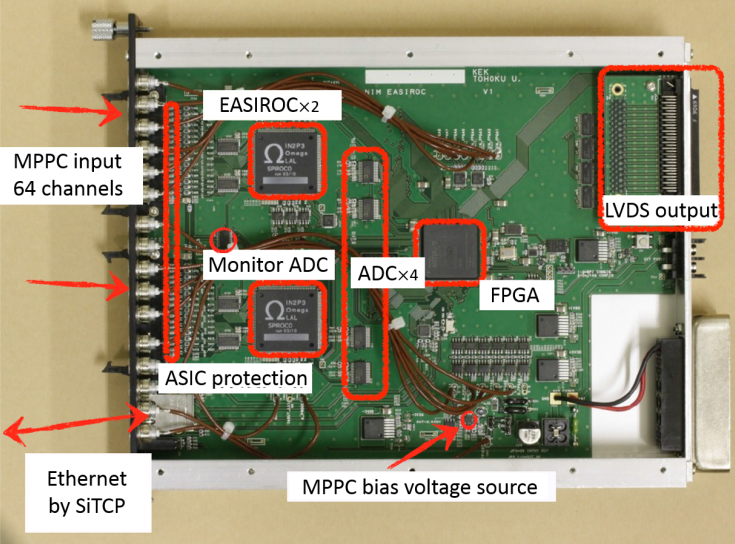
\includegraphics[width = 10.0cm, bb= 0 0 735 544]{2.png}
\end{center}
\caption{Side-view of NIM-EASIROC board}
\label{fig:}
\end{figure}

\begin{figure}[H]
\begin{center}
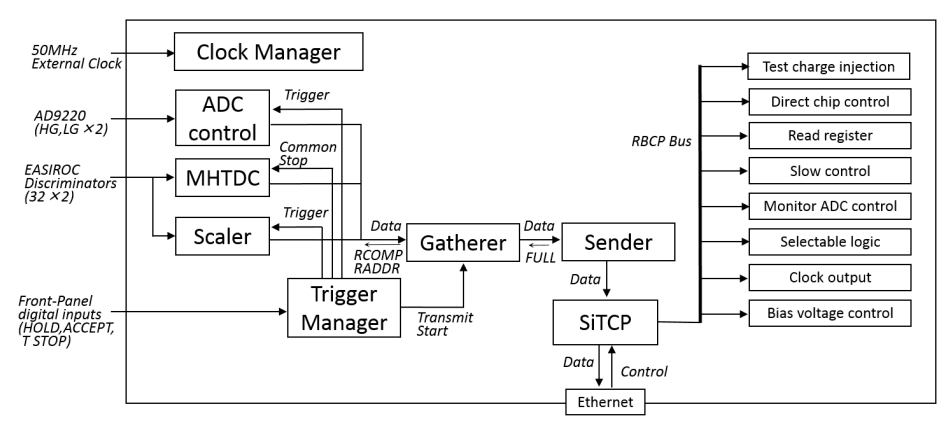
\includegraphics[width = 10.0cm, bb= 0 0 952 424]{3.png}
\end{center}
\caption{Circuit diagram of NIM-EASIROC board}
\label{fig:}
\end{figure}

\begin{figure}[H]
\begin{center}
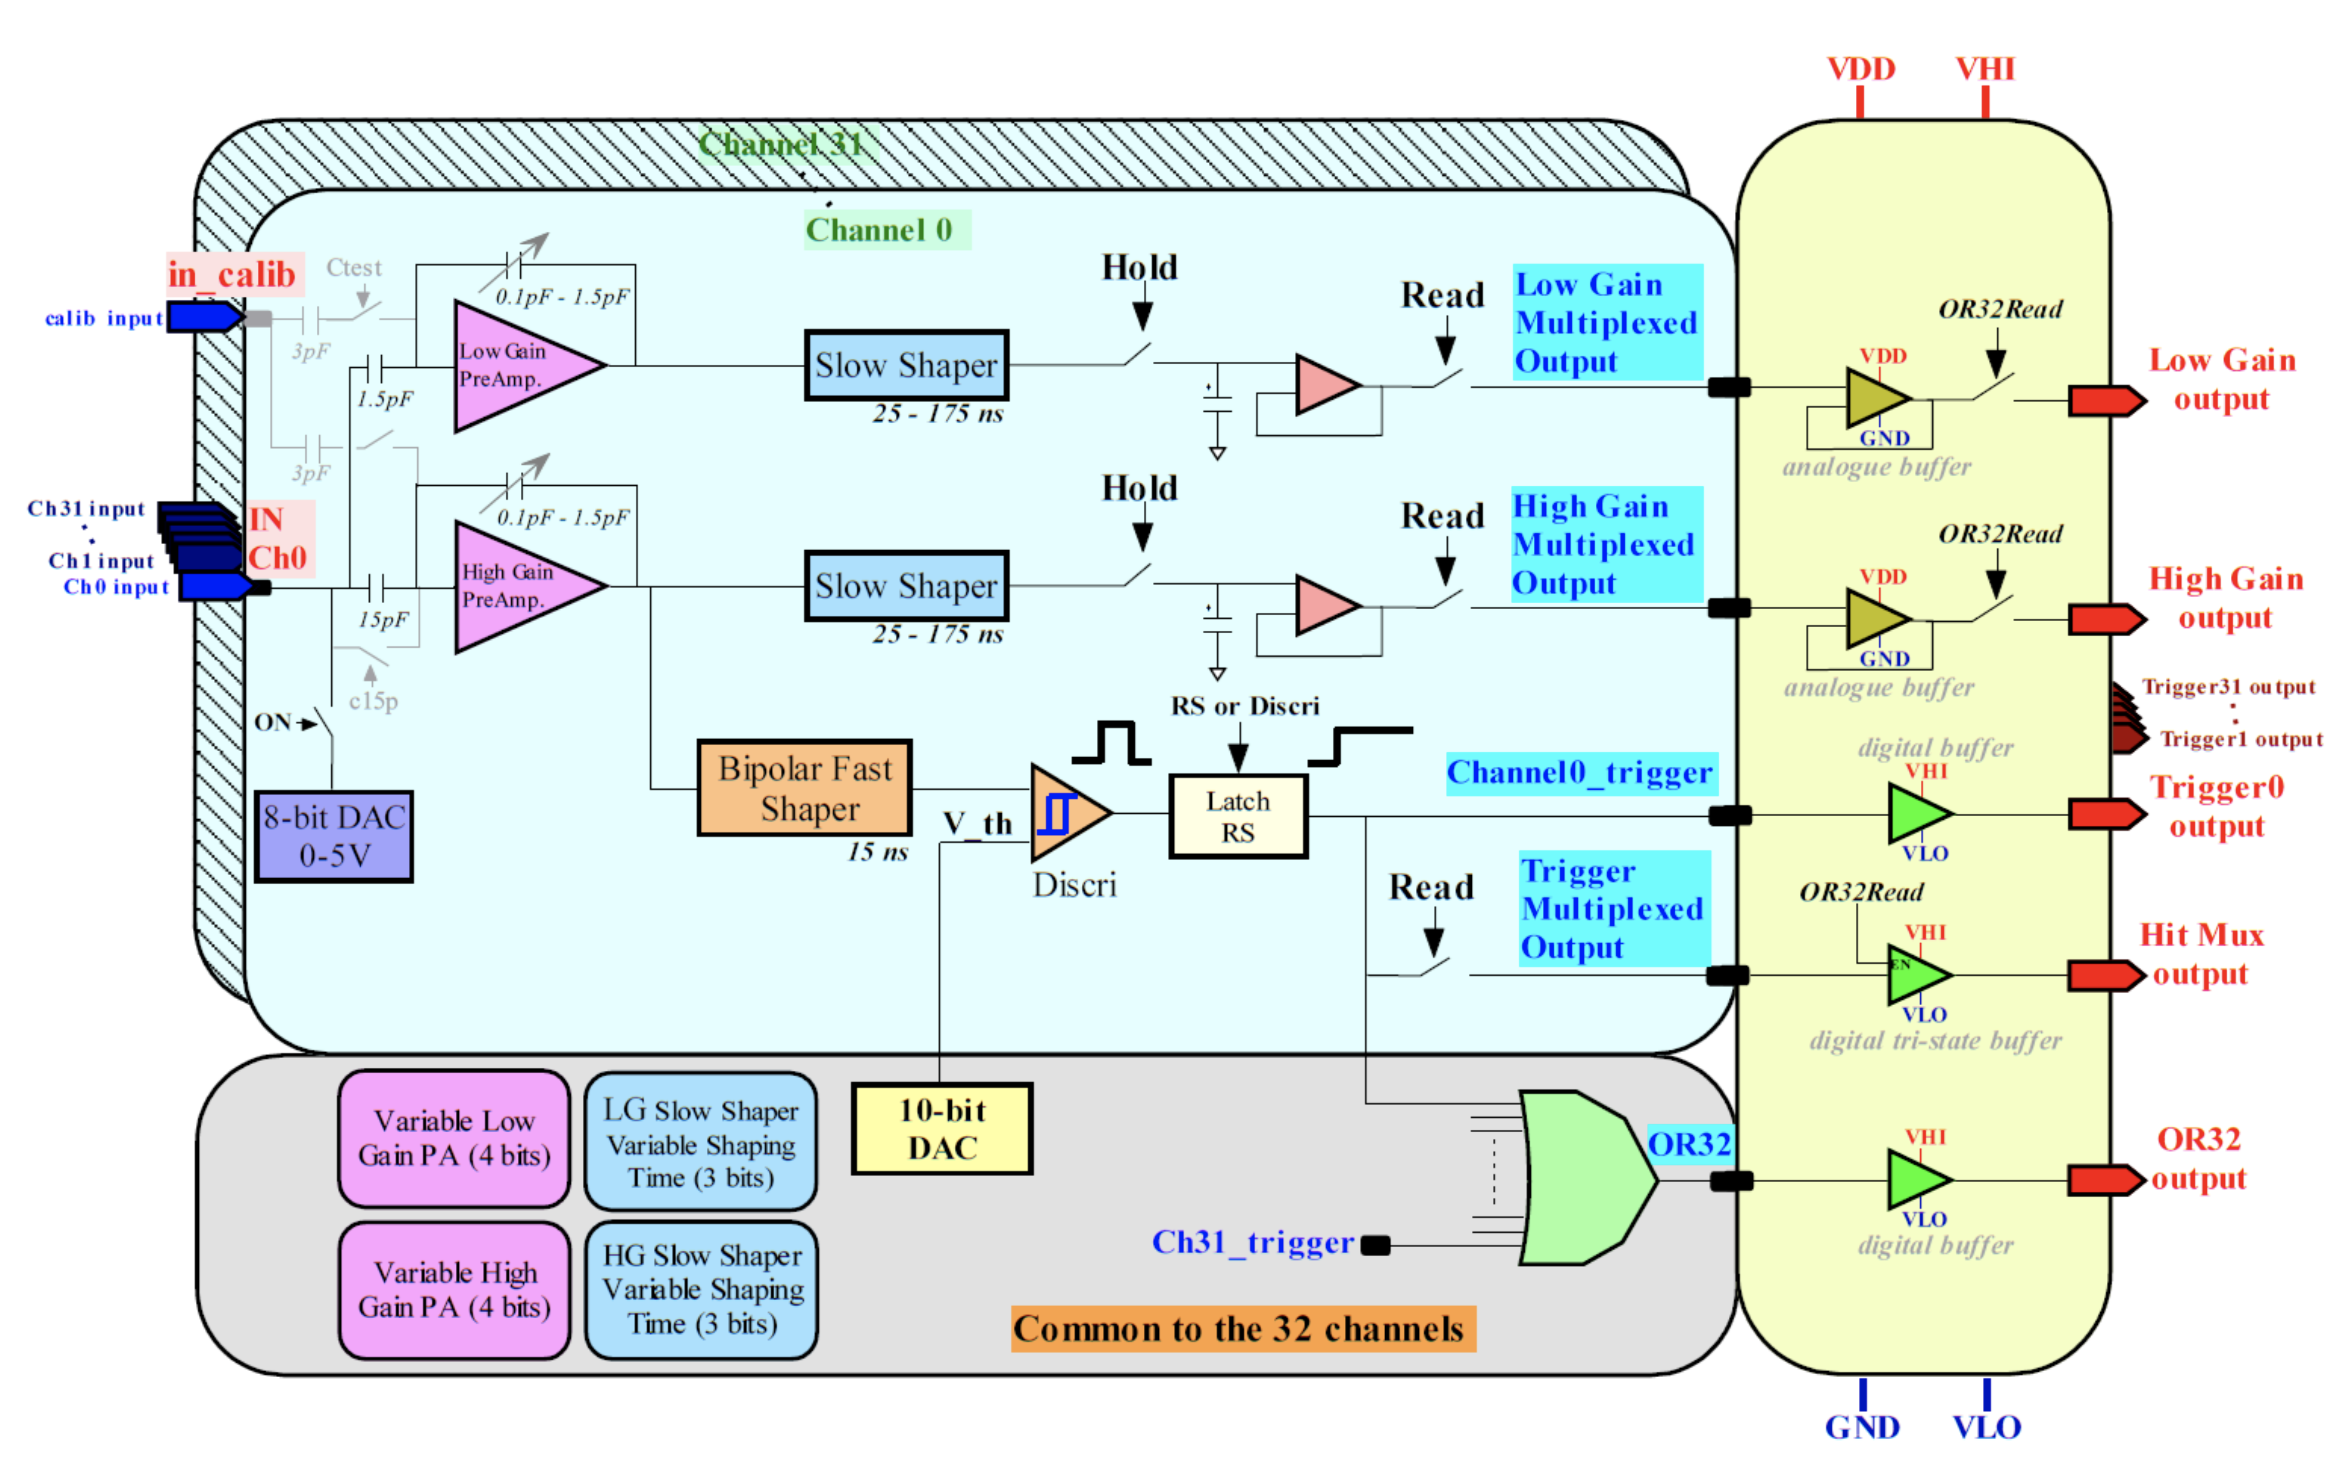
\includegraphics[width = 13.0cm, bb= 0 0 1167 735]{5.png}
\end{center}
\caption{Diagram of EASIROC chip}
\label{fig:}
\end{figure}

The way of converting the analog signal to the digital one is like this:
\begin{enumerate}
\item Integrate and amplify the charge by pre-amplifier which has two types of gain (low and high).
\item Send the pre-amplifier output to fast-shaper and slow-shaper.
\item Signal sent to the fast-shaper is shaped with the time constant 15 ns and converted to the digital signal if it is over the threshold of discriminator.
\item Signal sent to the slow-shaper is shaped with the time constant 25-175 ns and recorded its voltage value when it get HOLD signal.
\end{enumerate}

